% Options for packages loaded elsewhere
\PassOptionsToPackage{unicode}{hyperref}
\PassOptionsToPackage{hyphens}{url}
%
\documentclass[
  a4paper,
]{article}
\usepackage{lmodern}
\usepackage{amssymb,amsmath}
\usepackage{ifxetex,ifluatex}
\ifnum 0\ifxetex 1\fi\ifluatex 1\fi=0 % if pdftex
  \usepackage[T1]{fontenc}
  \usepackage[utf8]{inputenc}
  \usepackage{textcomp} % provide euro and other symbols
\else % if luatex or xetex
  \usepackage{unicode-math}
  \defaultfontfeatures{Scale=MatchLowercase}
  \defaultfontfeatures[\rmfamily]{Ligatures=TeX,Scale=1}
\fi
% Use upquote if available, for straight quotes in verbatim environments
\IfFileExists{upquote.sty}{\usepackage{upquote}}{}
\IfFileExists{microtype.sty}{% use microtype if available
  \usepackage[]{microtype}
  \UseMicrotypeSet[protrusion]{basicmath} % disable protrusion for tt fonts
}{}
\makeatletter
\@ifundefined{KOMAClassName}{% if non-KOMA class
  \IfFileExists{parskip.sty}{%
    \usepackage{parskip}
  }{% else
    \setlength{\parindent}{0pt}
    \setlength{\parskip}{6pt plus 2pt minus 1pt}}
}{% if KOMA class
  \KOMAoptions{parskip=half}}
\makeatother
\usepackage{xcolor}
\IfFileExists{xurl.sty}{\usepackage{xurl}}{} % add URL line breaks if available
\IfFileExists{bookmark.sty}{\usepackage{bookmark}}{\usepackage{hyperref}}
\hypersetup{
  pdftitle={Lab 5},
  pdfauthor={Emilio Dorigatti},
  hidelinks,
  pdfcreator={LaTeX via pandoc}}
\urlstyle{same} % disable monospaced font for URLs
\usepackage[margin=1in]{geometry}
\usepackage{color}
\usepackage{fancyvrb}
\newcommand{\VerbBar}{|}
\newcommand{\VERB}{\Verb[commandchars=\\\{\}]}
\DefineVerbatimEnvironment{Highlighting}{Verbatim}{commandchars=\\\{\}}
% Add ',fontsize=\small' for more characters per line
\usepackage{framed}
\definecolor{shadecolor}{RGB}{248,248,248}
\newenvironment{Shaded}{\begin{snugshade}}{\end{snugshade}}
\newcommand{\AlertTok}[1]{\textcolor[rgb]{0.94,0.16,0.16}{#1}}
\newcommand{\AnnotationTok}[1]{\textcolor[rgb]{0.56,0.35,0.01}{\textbf{\textit{#1}}}}
\newcommand{\AttributeTok}[1]{\textcolor[rgb]{0.77,0.63,0.00}{#1}}
\newcommand{\BaseNTok}[1]{\textcolor[rgb]{0.00,0.00,0.81}{#1}}
\newcommand{\BuiltInTok}[1]{#1}
\newcommand{\CharTok}[1]{\textcolor[rgb]{0.31,0.60,0.02}{#1}}
\newcommand{\CommentTok}[1]{\textcolor[rgb]{0.56,0.35,0.01}{\textit{#1}}}
\newcommand{\CommentVarTok}[1]{\textcolor[rgb]{0.56,0.35,0.01}{\textbf{\textit{#1}}}}
\newcommand{\ConstantTok}[1]{\textcolor[rgb]{0.00,0.00,0.00}{#1}}
\newcommand{\ControlFlowTok}[1]{\textcolor[rgb]{0.13,0.29,0.53}{\textbf{#1}}}
\newcommand{\DataTypeTok}[1]{\textcolor[rgb]{0.13,0.29,0.53}{#1}}
\newcommand{\DecValTok}[1]{\textcolor[rgb]{0.00,0.00,0.81}{#1}}
\newcommand{\DocumentationTok}[1]{\textcolor[rgb]{0.56,0.35,0.01}{\textbf{\textit{#1}}}}
\newcommand{\ErrorTok}[1]{\textcolor[rgb]{0.64,0.00,0.00}{\textbf{#1}}}
\newcommand{\ExtensionTok}[1]{#1}
\newcommand{\FloatTok}[1]{\textcolor[rgb]{0.00,0.00,0.81}{#1}}
\newcommand{\FunctionTok}[1]{\textcolor[rgb]{0.00,0.00,0.00}{#1}}
\newcommand{\ImportTok}[1]{#1}
\newcommand{\InformationTok}[1]{\textcolor[rgb]{0.56,0.35,0.01}{\textbf{\textit{#1}}}}
\newcommand{\KeywordTok}[1]{\textcolor[rgb]{0.13,0.29,0.53}{\textbf{#1}}}
\newcommand{\NormalTok}[1]{#1}
\newcommand{\OperatorTok}[1]{\textcolor[rgb]{0.81,0.36,0.00}{\textbf{#1}}}
\newcommand{\OtherTok}[1]{\textcolor[rgb]{0.56,0.35,0.01}{#1}}
\newcommand{\PreprocessorTok}[1]{\textcolor[rgb]{0.56,0.35,0.01}{\textit{#1}}}
\newcommand{\RegionMarkerTok}[1]{#1}
\newcommand{\SpecialCharTok}[1]{\textcolor[rgb]{0.00,0.00,0.00}{#1}}
\newcommand{\SpecialStringTok}[1]{\textcolor[rgb]{0.31,0.60,0.02}{#1}}
\newcommand{\StringTok}[1]{\textcolor[rgb]{0.31,0.60,0.02}{#1}}
\newcommand{\VariableTok}[1]{\textcolor[rgb]{0.00,0.00,0.00}{#1}}
\newcommand{\VerbatimStringTok}[1]{\textcolor[rgb]{0.31,0.60,0.02}{#1}}
\newcommand{\WarningTok}[1]{\textcolor[rgb]{0.56,0.35,0.01}{\textbf{\textit{#1}}}}
\usepackage{graphicx}
\makeatletter
\def\maxwidth{\ifdim\Gin@nat@width>\linewidth\linewidth\else\Gin@nat@width\fi}
\def\maxheight{\ifdim\Gin@nat@height>\textheight\textheight\else\Gin@nat@height\fi}
\makeatother
% Scale images if necessary, so that they will not overflow the page
% margins by default, and it is still possible to overwrite the defaults
% using explicit options in \includegraphics[width, height, ...]{}
\setkeys{Gin}{width=\maxwidth,height=\maxheight,keepaspectratio}
% Set default figure placement to htbp
\makeatletter
\def\fps@figure{htbp}
\makeatother
\setlength{\emergencystretch}{3em} % prevent overfull lines
\providecommand{\tightlist}{%
  \setlength{\itemsep}{0pt}\setlength{\parskip}{0pt}}
\setcounter{secnumdepth}{-\maxdimen} % remove section numbering
\usepackage{bbold}
\usepackage{tikz}
\usepackage[utf8]{inputenc}
\usetikzlibrary{snakes,arrows,shapes}
\ifluatex
  \usepackage{selnolig}  % disable illegal ligatures
\fi

\title{Lab 5}
\author{Emilio Dorigatti}
\date{2020-12-04}

\begin{document}
\maketitle

Welcome to the fifth lab. We will first implement a simple scalar
automatic differentiation engine to compute partial derivatives for us,
then do a theoretical exercise about L2 regularization.

\hypertarget{exercise-1}{%
\subsection{Exercise 1}\label{exercise-1}}

Modern deep learning frameworks compute gradients automatically, so that
you only need to define how to perform the forward pass in your code.
Under the hood, the framework constructs a computational graph based on
the operations you used. For example, consider the node:

\begin{equation}
4xy+e^{-y}
\label{eq:ex}
\end{equation}

It can be translated into a graph that looks like this:

\begin{figure}
\centering
\begin{tikzpicture}[>=latex',line join=bevel,]
  \node (a) at (27.0bp,234.0bp) [minimum size=1.25cm,draw,circle] {$4$};
  \node (e) at (99.0bp,162.0bp) [minimum size=1.25cm,draw,circle] {$\times$};
  \node (b) at (99.0bp,234.0bp) [minimum size=1.25cm,draw,circle] {$x$};
  \node (c) at (171.0bp,234.0bp) [minimum size=1.25cm,draw,circle] {$y$};
  \node (f) at (225.0bp,162.0bp) [minimum size=1.25cm,draw,circle] {$\times$};
  \node (g) at (153.0bp,90.0bp) [minimum size=1.25cm,draw,circle] {$\times$};
  \node (d) at (243.0bp,234.0bp) [minimum size=1.25cm,draw,circle] {$-1$};
  \node (h) at (225.0bp,90.0bp) [minimum size=1.25cm,draw,circle] {$\exp(\cdot)$};
  \node (i) at (189.0bp,18.0bp) [minimum size=1.25cm,draw,circle] {$+$};
  \draw [->] (a) ..controls (51.75bp,208.94bp) and (65.524bp,195.55bp)  .. (e);
  \draw [->] (b) ..controls (99.0bp,207.98bp) and (99.0bp,198.71bp)  .. (e);
  \draw [->] (c) ..controls (189.98bp,208.4bp) and (198.94bp,196.79bp)  .. (f);
  \draw [->] (c) ..controls (165.76bp,191.67bp) and (160.13bp,147.21bp)  .. (g);
  \draw [->] (d) ..controls (236.61bp,208.14bp) and (234.14bp,198.54bp)  .. (f);
  \draw [->] (e) ..controls (117.98bp,136.4bp) and (126.94bp,124.79bp)  .. (g);
  \draw [->] (f) ..controls (225.0bp,135.98bp) and (225.0bp,126.71bp)  .. (h);
  \draw [->] (g) ..controls (165.71bp,64.283bp) and (171.15bp,53.714bp)  .. (i);
  \draw [->] (h) ..controls (212.29bp,64.283bp) and (206.85bp,53.714bp)  .. (i);
\end{tikzpicture}
\caption{Computational graph representing Eq. \ref{eq:ex}.}
\label{fig:cg}
\end{figure}

Where we have ``leaf'' nodes at the top for variables and constants, and
``internal'' nodes for operations. To make things simpler, in this
exercise we will only work with scalar operations and scalar variables,
but what we are going to create could, in principle, be extended to work
with vectors and matrices. Section 6 of chapter 5 of the
\emph{Mathematics for Machine Learning} book
(\url{https://mml-book.github.io/}) is a good supplementary read.

A node is represented as a list with an attribute \texttt{op} to
indicate what kind of node it is. Leaf nodes are denoted as
\texttt{op="const"} or \texttt{op="var"}, with attributes to indicate
their value or name. Internal nodes have \texttt{op} set to the
operation they represent, and one or two attributes \texttt{x} and
\texttt{y} to denote their argument(s):

\begin{itemize}
\tightlist
\item
  \texttt{op="sum"} for Addition \(x+y\)
\item
  \texttt{op="sub"} for Subtraction \(x-y\)
\item
  \texttt{op="mul"} for Product \(x\cdot y\)
\item
  \texttt{op="div"} for Division \(x / y\)
\item
  \texttt{op="exp"} for Exponentiation \(e^x\)
\item
  \texttt{op="tanh"} for Hyperbolic tangent \(\tanh(x)\)
\item
  \texttt{op="log"} for Logarithm \(\log(x)\)
\end{itemize}

We first define some utility functions to easily create nodes:

\begin{Shaded}
\begin{Highlighting}[]
\CommentTok{\# node representing a constant}
\NormalTok{n.const }\OtherTok{=} \ControlFlowTok{function}\NormalTok{(value) }\FunctionTok{list}\NormalTok{(}\AttributeTok{op =} \StringTok{"const"}\NormalTok{, }\AttributeTok{value =}\NormalTok{ value)}

\CommentTok{\# node representing a variable}
\NormalTok{n.var }\OtherTok{=} \ControlFlowTok{function}\NormalTok{(name) }\FunctionTok{list}\NormalTok{(}\AttributeTok{op =} \StringTok{"var"}\NormalTok{, }\AttributeTok{name =}\NormalTok{ name)}

\CommentTok{\# nodes for binary operations}
\NormalTok{n.sum }\OtherTok{=} \ControlFlowTok{function}\NormalTok{(x, y) }\FunctionTok{list}\NormalTok{(}\AttributeTok{op =} \StringTok{"sum"}\NormalTok{, }\AttributeTok{x =}\NormalTok{ x, }\AttributeTok{y =}\NormalTok{ y)}
\NormalTok{n.sub }\OtherTok{=} \ControlFlowTok{function}\NormalTok{(x, y) }\FunctionTok{list}\NormalTok{(}\AttributeTok{op =} \StringTok{"sub"}\NormalTok{, }\AttributeTok{x =}\NormalTok{ x, }\AttributeTok{y =}\NormalTok{ y)}
\NormalTok{n.mul }\OtherTok{=} \ControlFlowTok{function}\NormalTok{(x, y) }\FunctionTok{list}\NormalTok{(}\AttributeTok{op =} \StringTok{"mul"}\NormalTok{, }\AttributeTok{x =}\NormalTok{ x, }\AttributeTok{y =}\NormalTok{ y)}
\NormalTok{n.div }\OtherTok{=} \ControlFlowTok{function}\NormalTok{(x, y) }\FunctionTok{list}\NormalTok{(}\AttributeTok{op =} \StringTok{"div"}\NormalTok{, }\AttributeTok{x =}\NormalTok{ x, }\AttributeTok{y =}\NormalTok{ y)}

\CommentTok{\# nodes for functions}
\NormalTok{n.exp }\OtherTok{=} \ControlFlowTok{function}\NormalTok{(x) }\FunctionTok{list}\NormalTok{(}\AttributeTok{op =} \StringTok{"exp"}\NormalTok{, }\AttributeTok{x =}\NormalTok{ x)}
\NormalTok{n.log }\OtherTok{=} \ControlFlowTok{function}\NormalTok{(x) }\FunctionTok{list}\NormalTok{(}\AttributeTok{op =} \StringTok{"log"}\NormalTok{, }\AttributeTok{x =}\NormalTok{ x)}
\NormalTok{n.tanh }\OtherTok{=} \ControlFlowTok{function}\NormalTok{(x) }\FunctionTok{list}\NormalTok{(}\AttributeTok{op =} \StringTok{"tanh"}\NormalTok{, }\AttributeTok{x =}\NormalTok{ x)}

\CommentTok{\# now define the graph computing Eq. 1 and show in Fig. 1}
\NormalTok{x }\OtherTok{=} \FunctionTok{n.var}\NormalTok{(}\StringTok{"x"}\NormalTok{)}
\NormalTok{y }\OtherTok{=} \FunctionTok{n.var}\NormalTok{(}\StringTok{"y"}\NormalTok{)}

\NormalTok{z }\OtherTok{=} \FunctionTok{n.sum}\NormalTok{(}
  \FunctionTok{n.mul}\NormalTok{(}
     \FunctionTok{n.mul}\NormalTok{(}
        \FunctionTok{n.const}\NormalTok{(}\DecValTok{4}\NormalTok{),}
\NormalTok{        x),}
\NormalTok{     y),}
  \FunctionTok{n.exp}\NormalTok{(}
     \FunctionTok{n.mul}\NormalTok{(}
        \FunctionTok{n.const}\NormalTok{(}\SpecialCharTok{{-}}\DecValTok{1}\NormalTok{),}
\NormalTok{        y)))}

\NormalTok{z}
\end{Highlighting}
\end{Shaded}

\begin{verbatim}
## $op
## [1] "sum"
## 
## $x
## $x$op
## [1] "mul"
## 
## $x$x
## $x$x$op
## [1] "mul"
## 
## $x$x$x
## $x$x$x$op
## [1] "const"
## 
## $x$x$x$value
## [1] 4
## 
## 
## $x$x$y
## $x$x$y$op
## [1] "var"
## 
## $x$x$y$name
## [1] "x"
## 
## 
## 
## $x$y
## $x$y$op
## [1] "var"
## 
## $x$y$name
## [1] "y"
## 
## 
## 
## $y
## $y$op
## [1] "exp"
## 
## $y$x
## $y$x$op
## [1] "mul"
## 
## $y$x$x
## $y$x$x$op
## [1] "const"
## 
## $y$x$x$value
## [1] -1
## 
## 
## $y$x$y
## $y$x$y$op
## [1] "var"
## 
## $y$x$y$name
## [1] "y"
\end{verbatim}

This structure of nested lists contains the computational graph for the
node above. Now, we can write code to manipulate this expression as we
please. In the course of this exercise, we will see how:

\begin{enumerate}
\def\labelenumi{\arabic{enumi}.}
\tightlist
\item
  Print an expression,
\item
  Compute its value, given the values of the variables involved,
\item
  Differentiate it to automatically find partial derivatives with
  respect to any given variable,
\item
  Transform it into simpler expressions that are cheaper to handle, and
\item
  Write code to train a neural network without getting our hands dirty
  with derivatives ever again.
\end{enumerate}

\hypertarget{printing-an-expression}{%
\subsubsection{Printing an expression}\label{printing-an-expression}}

First, since it is quite hard to understand the node from the
representation above, let us write a function to convert a computational
graph into a string representation that is easier to understand. For
example, the expression \(x+2y\) should be converted to

\begin{Shaded}
\begin{Highlighting}[]
\FunctionTok{c}\NormalTok{(}\StringTok{"("}\NormalTok{, }\StringTok{"x"}\NormalTok{, }\StringTok{"+"}\NormalTok{, }\StringTok{"("}\NormalTok{, }\StringTok{"2"}\NormalTok{, }\StringTok{"*"}\NormalTok{, }\StringTok{"y"}\NormalTok{, }\StringTok{")"}\NormalTok{, }\StringTok{")"}\NormalTok{)}
\end{Highlighting}
\end{Shaded}

Which can be printed easily using \texttt{cat}, resulting in
\texttt{(\ x\ +\ (\ 2\ *\ y\ )\ )}.

Such a function should be \emph{recursive}. This means that when
simplifying a complicated expression it will call itself on each
constituting piece of that expression, and ``assemble'' the results
together. Conceptually, the procedure is similar to the factorial
operation, which is recursively defined in terms of the factorial of a
smaller number:

\begin{equation}
n!=\begin{cases}
1 & \text{if }n < 1 \\
n\cdot(n-1)! & \text{otherwise}
\end{cases}
\end{equation}

This definition can be converted into R as:

\begin{Shaded}
\begin{Highlighting}[]
\NormalTok{factorial }\OtherTok{=} \ControlFlowTok{function}\NormalTok{(n) \{}
  \ControlFlowTok{if}\NormalTok{(n }\SpecialCharTok{\textless{}} \DecValTok{1}\NormalTok{) \{}
    \DecValTok{1}
\NormalTok{  \}}
  \ControlFlowTok{else}\NormalTok{ \{}
\NormalTok{    n }\SpecialCharTok{*} \FunctionTok{factorial}\NormalTok{(n }\SpecialCharTok{{-}} \DecValTok{1}\NormalTok{)}
\NormalTok{  \}}
\NormalTok{\}}

\FunctionTok{factorial}\NormalTok{(}\DecValTok{4}\NormalTok{)}
\end{Highlighting}
\end{Shaded}

\begin{verbatim}
## [1] 24
\end{verbatim}

In a similar way, the function \texttt{to.string} below should call
itself to ``stringify'' the operands on an operation, then merge these
representations into a single string for the whole operation. This basic
skeleton of recursively navigating the computational graph will be used
throughout the exercise.

\begin{Shaded}
\begin{Highlighting}[]
\NormalTok{to.string }\OtherTok{=} \ControlFlowTok{function}\NormalTok{(node) \{}
  \CommentTok{\# return a vector of strings representing each parts of the node}
  
  \ControlFlowTok{if}\NormalTok{(node}\SpecialCharTok{$}\NormalTok{op }\SpecialCharTok{==} \StringTok{"const"}\NormalTok{) \{}
    \CommentTok{\# the string representation of a constant is its value}
    \FunctionTok{c}\NormalTok{(node}\SpecialCharTok{$}\NormalTok{value)}
\NormalTok{  \}}
  \ControlFlowTok{else} \ControlFlowTok{if}\NormalTok{(node}\SpecialCharTok{$}\NormalTok{op }\SpecialCharTok{==} \StringTok{"var"}\NormalTok{) \{}
    \CommentTok{\# the string representation of a variable is its name}
    \FunctionTok{c}\NormalTok{(node}\SpecialCharTok{$}\NormalTok{name)}
\NormalTok{  \}}
  \ControlFlowTok{else} \ControlFlowTok{if}\NormalTok{(node}\SpecialCharTok{$}\NormalTok{op }\SpecialCharTok{\%in\%} \FunctionTok{c}\NormalTok{(}\StringTok{"sum"}\NormalTok{, }\StringTok{"sub"}\NormalTok{, }\StringTok{"mul"}\NormalTok{, }\StringTok{"div"}\NormalTok{)) \{}
    \CommentTok{\# find the string representation of the operation}
\NormalTok{    operator }\OtherTok{=} \FunctionTok{list}\NormalTok{(}
      \AttributeTok{sum =} \StringTok{"+"}\NormalTok{, }\AttributeTok{sub =} \StringTok{"{-}"}\NormalTok{, }\AttributeTok{mul =} \StringTok{"*"}\NormalTok{, }\AttributeTok{div =} \StringTok{"/"}
\NormalTok{    )[[node}\SpecialCharTok{$}\NormalTok{op]]}
    
\NormalTok{    string\_x }\OtherTok{=}\NormalTok{ (}
      \CommentTok{\# }\AlertTok{TODO}\CommentTok{ use the function \textasciigrave{}to.string\textasciigrave{} to find the string}
      \CommentTok{\# representation of the left part}
\NormalTok{    )}
    
\NormalTok{    string\_y }\OtherTok{=}\NormalTok{ (}
      \CommentTok{\# }\AlertTok{TODO}\CommentTok{ use the function \textasciigrave{}to.string\textasciigrave{} to find the string}
      \CommentTok{\#  representation of the right part}
\NormalTok{    )}
    
    \FunctionTok{c}\NormalTok{(}
      \StringTok{"("}\NormalTok{,}
      \CommentTok{\# }\AlertTok{TODO}\CommentTok{ return the string representation of this operation}
      \CommentTok{\#  by "assembling" the individual pieces}
      \StringTok{")"}
\NormalTok{    )}
\NormalTok{  \}}
  \ControlFlowTok{else} \ControlFlowTok{if}\NormalTok{(node}\SpecialCharTok{$}\NormalTok{op }\SpecialCharTok{\%in\%} \FunctionTok{c}\NormalTok{(}\StringTok{"tanh"}\NormalTok{, }\StringTok{"exp"}\NormalTok{, }\StringTok{"log"}\NormalTok{)) \{}
    \FunctionTok{c}\NormalTok{(}
      \CommentTok{\# }\AlertTok{TODO}\CommentTok{ return the string representation of the function name}
      \CommentTok{\# and its argument}
\NormalTok{    )}
\NormalTok{  \}}
  \ControlFlowTok{else}\NormalTok{ \{}
    \FunctionTok{stop}\NormalTok{(}\FunctionTok{c}\NormalTok{(}\StringTok{"unknown node: "}\NormalTok{, node}\SpecialCharTok{$}\NormalTok{op))}
\NormalTok{  \}}
\NormalTok{\}}

\NormalTok{print.node }\OtherTok{=} \ControlFlowTok{function}\NormalTok{(node) \{}
  \FunctionTok{cat}\NormalTok{(}\FunctionTok{to.string}\NormalTok{(node), }\StringTok{"}\SpecialCharTok{\textbackslash{}n}\StringTok{"}\NormalTok{)}
\NormalTok{\}}

\FunctionTok{print.node}\NormalTok{(z)}
\end{Highlighting}
\end{Shaded}

This is much simpler to read!

\hypertarget{computing-the-value-of-an-expression}{%
\subsubsection{Computing the value of an
expression}\label{computing-the-value-of-an-expression}}

We can now write a function to compute the value of an expression given
values for the variables. This function should be recursive too, like
\texttt{to.string} above.

\begin{Shaded}
\begin{Highlighting}[]
\NormalTok{compute }\OtherTok{=} \ControlFlowTok{function}\NormalTok{(node, var\_values) \{}
  \CommentTok{\# compute the numerical result of the node using the provided variable values}
  
  \ControlFlowTok{if}\NormalTok{(node}\SpecialCharTok{$}\NormalTok{op }\SpecialCharTok{==} \StringTok{"const"}\NormalTok{) \{}
    \CommentTok{\# the value of a constant is its value}
\NormalTok{    node}\SpecialCharTok{$}\NormalTok{value}
\NormalTok{  \}}
  \ControlFlowTok{else} \ControlFlowTok{if}\NormalTok{(node}\SpecialCharTok{$}\NormalTok{op }\SpecialCharTok{==} \StringTok{"var"}\NormalTok{) \{}
    \CommentTok{\# read the value of the variable from the list}
\NormalTok{    val }\OtherTok{=}\NormalTok{ var\_values[[node}\SpecialCharTok{$}\NormalTok{name]]}
    \ControlFlowTok{if}\NormalTok{(}\FunctionTok{is.null}\NormalTok{(val)) \{}
      \FunctionTok{stop}\NormalTok{(}\FunctionTok{c}\NormalTok{(}\StringTok{"value not defined or NULL for variable "}\NormalTok{, node}\SpecialCharTok{$}\NormalTok{name))}
\NormalTok{    \}}
    \ControlFlowTok{else}\NormalTok{ \{}
\NormalTok{      val}
\NormalTok{    \}}
\NormalTok{  \}}
  \ControlFlowTok{else} \ControlFlowTok{if}\NormalTok{(node}\SpecialCharTok{$}\NormalTok{op }\SpecialCharTok{==} \StringTok{"sum"}\NormalTok{) \{}
\NormalTok{    value\_x }\OtherTok{=}\NormalTok{ (}
      \CommentTok{\# }\AlertTok{TODO}\CommentTok{ compute the value for the right operand}
\NormalTok{    )}
    
\NormalTok{    value\_y }\OtherTok{=}\NormalTok{ (}
      \CommentTok{\# }\AlertTok{TODO}\CommentTok{ compute the value for the right operand}
\NormalTok{    )}
    
    \CommentTok{\# add the values and return the result}
\NormalTok{    value\_x }\SpecialCharTok{+}\NormalTok{ value\_y}
\NormalTok{  \}}
  \ControlFlowTok{else} \ControlFlowTok{if}\NormalTok{(node}\SpecialCharTok{$}\NormalTok{op }\SpecialCharTok{==} \StringTok{"sub"}\NormalTok{) \{}
    \CommentTok{\# }\AlertTok{TODO}\CommentTok{ perform the subtraction x {-} y}
\NormalTok{  \}}
  \ControlFlowTok{else} \ControlFlowTok{if}\NormalTok{(node}\SpecialCharTok{$}\NormalTok{op }\SpecialCharTok{==} \StringTok{"mul"}\NormalTok{) \{}
    \CommentTok{\# }\AlertTok{TODO}\CommentTok{ perform the product x * y}
\NormalTok{  \}}
  \ControlFlowTok{else} \ControlFlowTok{if}\NormalTok{(node}\SpecialCharTok{$}\NormalTok{op }\SpecialCharTok{==} \StringTok{"div"}\NormalTok{) \{}
    \CommentTok{\# }\AlertTok{TODO}\CommentTok{ perform the division x / y}
\NormalTok{  \}}
  \ControlFlowTok{else} \ControlFlowTok{if}\NormalTok{(node}\SpecialCharTok{$}\NormalTok{op }\SpecialCharTok{==} \StringTok{"tanh"}\NormalTok{) \{}
    \CommentTok{\# }\AlertTok{TODO}\CommentTok{ compute the hyperbolic tangent of x}
\NormalTok{  \}}
  \ControlFlowTok{else} \ControlFlowTok{if}\NormalTok{(node}\SpecialCharTok{$}\NormalTok{op }\SpecialCharTok{==} \StringTok{"exp"}\NormalTok{) \{}
    \CommentTok{\# }\AlertTok{TODO}\CommentTok{ compute the exponential of x}
\NormalTok{  \}}
  \ControlFlowTok{else} \ControlFlowTok{if}\NormalTok{(node}\SpecialCharTok{$}\NormalTok{op }\SpecialCharTok{==} \StringTok{"log"}\NormalTok{) \{}
    \CommentTok{\# }\AlertTok{TODO}\CommentTok{ compute the logarithm of x}
\NormalTok{  \}}
  \ControlFlowTok{else}\NormalTok{ \{}
    \FunctionTok{stop}\NormalTok{(}\FunctionTok{c}\NormalTok{(}\StringTok{"unknown node: "}\NormalTok{, node}\SpecialCharTok{$}\NormalTok{op))}
\NormalTok{  \}}
\NormalTok{\}}

\FunctionTok{compute}\NormalTok{(z, }\FunctionTok{list}\NormalTok{(}\AttributeTok{x =} \DecValTok{2}\NormalTok{, }\AttributeTok{y =} \DecValTok{3}\NormalTok{))}
\end{Highlighting}
\end{Shaded}

The result that we expect is, of course:

\begin{Shaded}
\begin{Highlighting}[]
\DecValTok{4} \SpecialCharTok{*} \DecValTok{2} \SpecialCharTok{*} \DecValTok{3} \SpecialCharTok{+} \FunctionTok{exp}\NormalTok{(}\SpecialCharTok{{-}}\DecValTok{3}\NormalTok{)}
\end{Highlighting}
\end{Shaded}

\begin{verbatim}
## [1] 24.04979
\end{verbatim}

\hypertarget{differentiating-an-expression}{%
\subsubsection{Differentiating an
expression}\label{differentiating-an-expression}}

We can finally see how to differentiate an expression with respect to a
variable. We do this again through a recursive function that
differentiates each argument and merges the result. Note that this
function should return a new computational graph that contains the
operations necessary to compute the partial derivative we are interested
in.

Remember to use the chain rule where appropriate!

\begin{Shaded}
\begin{Highlighting}[]
\NormalTok{differentiate }\OtherTok{=} \ControlFlowTok{function}\NormalTok{(node, variable) \{}
  \CommentTok{\# differentiate the given expression with respect to the given variable}
  \CommentTok{\#}
  \CommentTok{\# VERY IMPORTANT: this function returns a graph, which can only contain nodes.}
  \CommentTok{\# Therefore, you must use the functions n.const, n.sum, etc., instead of normal}
  \CommentTok{\# numbers and operations.}
  
  \ControlFlowTok{if}\NormalTok{(node}\SpecialCharTok{$}\NormalTok{op }\SpecialCharTok{==} \StringTok{"const"}\NormalTok{) \{}
    \CommentTok{\# derivative of a constant is always zero}
    \FunctionTok{n.const}\NormalTok{(}\DecValTok{0}\NormalTok{)}
\NormalTok{  \}}
  \ControlFlowTok{else} \ControlFlowTok{if}\NormalTok{(node}\SpecialCharTok{$}\NormalTok{op }\SpecialCharTok{==} \StringTok{"var"}\NormalTok{) \{}
    \ControlFlowTok{if}\NormalTok{(node}\SpecialCharTok{$}\NormalTok{name }\SpecialCharTok{==}\NormalTok{ variable) \{}
      \CommentTok{\# derivative is one if we are differentiating with respect to this variable}
      \FunctionTok{n.const}\NormalTok{(}\DecValTok{1}\NormalTok{)}
\NormalTok{    \}}
    \ControlFlowTok{else}\NormalTok{ \{}
      \CommentTok{\# or zero if we are differentiating with respect to a different variable}
      \FunctionTok{n.const}\NormalTok{(}\DecValTok{0}\NormalTok{)}
\NormalTok{    \}}
\NormalTok{  \}}
  \CommentTok{\# call the right function depending on what type of node we are processing}
  \ControlFlowTok{else} \ControlFlowTok{if}\NormalTok{(node}\SpecialCharTok{$}\NormalTok{op }\SpecialCharTok{==} \StringTok{"sum"}\NormalTok{) \{}
    \FunctionTok{differentiate.sum}\NormalTok{(node, variable)}
\NormalTok{  \}}
  \ControlFlowTok{else} \ControlFlowTok{if}\NormalTok{(node}\SpecialCharTok{$}\NormalTok{op }\SpecialCharTok{==} \StringTok{"sub"}\NormalTok{) \{}
    \FunctionTok{differentiate.sub}\NormalTok{(node, variable)}
\NormalTok{  \}}
  \ControlFlowTok{else} \ControlFlowTok{if}\NormalTok{(node}\SpecialCharTok{$}\NormalTok{op }\SpecialCharTok{==} \StringTok{"mul"}\NormalTok{) \{}
    \FunctionTok{differentiate.mul}\NormalTok{(node, variable)}
\NormalTok{  \}}
  \ControlFlowTok{else} \ControlFlowTok{if}\NormalTok{(node}\SpecialCharTok{$}\NormalTok{op }\SpecialCharTok{==} \StringTok{"div"}\NormalTok{) \{}
    \FunctionTok{differentiate.div}\NormalTok{(node, variable)}
\NormalTok{  \}}
  \ControlFlowTok{else} \ControlFlowTok{if}\NormalTok{(node}\SpecialCharTok{$}\NormalTok{op }\SpecialCharTok{==} \StringTok{"tanh"}\NormalTok{) \{}
    \FunctionTok{differentiate.tanh}\NormalTok{(node, variable)}
\NormalTok{  \}}
  \ControlFlowTok{else} \ControlFlowTok{if}\NormalTok{(node}\SpecialCharTok{$}\NormalTok{op }\SpecialCharTok{==} \StringTok{"exp"}\NormalTok{) \{}
    \FunctionTok{differentiate.exp}\NormalTok{(node, variable)}
\NormalTok{  \}}
  \ControlFlowTok{else} \ControlFlowTok{if}\NormalTok{(node}\SpecialCharTok{$}\NormalTok{op }\SpecialCharTok{==} \StringTok{"log"}\NormalTok{) \{}
    \FunctionTok{differentiate.log}\NormalTok{(node, variable)}
\NormalTok{  \}}
  \ControlFlowTok{else}\NormalTok{ \{}
    \FunctionTok{stop}\NormalTok{(}\FunctionTok{c}\NormalTok{(}\StringTok{"unknown node: "}\NormalTok{, node}\SpecialCharTok{$}\NormalTok{op))}
\NormalTok{  \}}
\NormalTok{\}}

\NormalTok{differentiate.sum }\OtherTok{=} \ControlFlowTok{function}\NormalTok{(node, variable) \{}
\NormalTok{  diff\_x }\OtherTok{=}\NormalTok{ (}
    \CommentTok{\# }\AlertTok{TODO}\CommentTok{ differentiate the left part}
\NormalTok{  )}
\NormalTok{  diff\_y }\OtherTok{=}\NormalTok{ (}
    \CommentTok{\# }\AlertTok{TODO}\CommentTok{ differentiate the right part}
\NormalTok{  )}
  
  \CommentTok{\# return a new node that sums the derivatives of the left and right part}
  \CommentTok{\#}
  \CommentTok{\# note that we are returning a new graph node that connects the two}
  \CommentTok{\# graphs representing the derivatives of the left and right parts}
  \FunctionTok{n.sum}\NormalTok{(diff\_x, diff\_y)}
\NormalTok{\}}

\NormalTok{differentiate.sub }\OtherTok{=} \ControlFlowTok{function}\NormalTok{(node, variable) \{}
  \CommentTok{\# }\AlertTok{TODO}\CommentTok{ differentiate the subtraction x {-} y}
\NormalTok{\}}

\NormalTok{differentiate.mul }\OtherTok{=} \ControlFlowTok{function}\NormalTok{(node, variable) \{}
  \CommentTok{\# }\AlertTok{TODO}\CommentTok{ differentiate the product x * y}
\NormalTok{\}}

\NormalTok{differentiate.div }\OtherTok{=} \ControlFlowTok{function}\NormalTok{(node, variable) \{}
  \CommentTok{\# }\AlertTok{TODO}\CommentTok{ differentiate the quotient x / y}
\NormalTok{\}}

\NormalTok{differentiate.tanh }\OtherTok{=} \ControlFlowTok{function}\NormalTok{(node, variable) \{}
  \CommentTok{\# }\AlertTok{TODO}\CommentTok{ differentiate tanh(x)}
\NormalTok{\}}

\NormalTok{differentiate.exp }\OtherTok{=} \ControlFlowTok{function}\NormalTok{(node, variable) \{}
  \CommentTok{\# }\AlertTok{TODO}\CommentTok{ differentiate exp(x)}
\NormalTok{\}}


\NormalTok{differentiate.log }\OtherTok{=} \ControlFlowTok{function}\NormalTok{(node, variable) \{}
  \CommentTok{\# }\AlertTok{TODO}\CommentTok{ differentiate log(x)}
\NormalTok{\}}

\NormalTok{dz }\OtherTok{=} \FunctionTok{differentiate}\NormalTok{(z, }\StringTok{"x"}\NormalTok{)}
\FunctionTok{print.node}\NormalTok{(dz)}
\end{Highlighting}
\end{Shaded}

This looks a bit complicated, but by applying some trivial
simplifications we see it is correct:

\begin{align*}
& ( ( ( ( ( 0 \cdot x ) + ( 4 \cdot 1 ) ) \cdot y ) + ( ( 4 \cdot x ) \cdot 0 ) ) + ( exp ( ( -1 \cdot y ) ) \cdot ( ( 0 \cdot y ) + ( -1 \cdot 0 ) ) ) )  \\
&\qquad= ( ( ( 0 + 4 ) \cdot y ) + 0 ) + ( exp ( ( -1 \cdot y ) ) \cdot ( 0 + 0 ) ) ) \\
&\qquad= ( 4 \cdot y ) + ( exp ( ( -1 \cdot y ) ) \cdot 0 ) ) \\
&\qquad= ( 4 \cdot y ) + 0 \\
&\qquad= 4 \cdot y \\
&\qquad= \frac{\text{d}}{\text{d}x} \left(4xy+e^{-y}\right)
\end{align*}

These simplification rules are trivial arithmetic identities:

\begin{itemize}
\tightlist
\item
  \(0+x=x\)
\item
  \(0\cdot x=0\)
\item
  \(1\cdot x=x\)
\item
  \(0/x=0\)
\end{itemize}

Let us write a function that uses these identities to automatically
simplify \texttt{dz} in the same way we just did. As with
differentiation, this function should return a new computational graph.

\begin{Shaded}
\begin{Highlighting}[]
\NormalTok{is.zero }\OtherTok{=} \ControlFlowTok{function}\NormalTok{(node) \{}
  \CommentTok{\# returns TRUE iff the node is the constant "0"}
\NormalTok{  node}\SpecialCharTok{$}\NormalTok{op }\SpecialCharTok{==} \StringTok{"const"} \SpecialCharTok{\&\&}\NormalTok{ node}\SpecialCharTok{$}\NormalTok{value }\SpecialCharTok{==} \DecValTok{0}
\NormalTok{\}}

\NormalTok{is.one }\OtherTok{=} \ControlFlowTok{function}\NormalTok{(node) \{}
  \CommentTok{\# returns TRUE iff the node is the constant "1"}
\NormalTok{  node}\SpecialCharTok{$}\NormalTok{op }\SpecialCharTok{==} \StringTok{"const"} \SpecialCharTok{\&\&}\NormalTok{ node}\SpecialCharTok{$}\NormalTok{value }\SpecialCharTok{==} \DecValTok{1}
\NormalTok{\}}

\NormalTok{simplify }\OtherTok{=} \ControlFlowTok{function}\NormalTok{(node) \{}
  \CommentTok{\# simplifies the provided node, returning a new computational graph}
  
  \ControlFlowTok{if}\NormalTok{(node}\SpecialCharTok{$}\NormalTok{op }\SpecialCharTok{\%in\%} \FunctionTok{c}\NormalTok{(}\StringTok{"const"}\NormalTok{, }\StringTok{"var"}\NormalTok{)) \{}
    \CommentTok{\# constants and variables cannot be simplified}
\NormalTok{    node}
\NormalTok{  \}}
  \CommentTok{\# call the right function depending on what type of node we are processing}
  \ControlFlowTok{else} \ControlFlowTok{if}\NormalTok{(node}\SpecialCharTok{$}\NormalTok{op }\SpecialCharTok{==} \StringTok{"sum"}\NormalTok{) \{}
    \FunctionTok{simplify.sum}\NormalTok{(node)}
\NormalTok{  \}}
  \ControlFlowTok{else} \ControlFlowTok{if}\NormalTok{(node}\SpecialCharTok{$}\NormalTok{op }\SpecialCharTok{==} \StringTok{"sub"}\NormalTok{) \{}
    \FunctionTok{simplify.sub}\NormalTok{(node)}
\NormalTok{  \}}
  \ControlFlowTok{else} \ControlFlowTok{if}\NormalTok{(node}\SpecialCharTok{$}\NormalTok{op }\SpecialCharTok{==} \StringTok{"mul"}\NormalTok{) \{}
    \FunctionTok{simplify.mul}\NormalTok{(node)}
\NormalTok{  \}}
  \ControlFlowTok{else} \ControlFlowTok{if}\NormalTok{(node}\SpecialCharTok{$}\NormalTok{op }\SpecialCharTok{==} \StringTok{"div"}\NormalTok{) \{}
    \FunctionTok{simplify.div}\NormalTok{(node)}
\NormalTok{  \}}
  \ControlFlowTok{else} \ControlFlowTok{if}\NormalTok{(node}\SpecialCharTok{$}\NormalTok{op }\SpecialCharTok{==} \StringTok{"tanh"}\NormalTok{) \{}
    \FunctionTok{simplify.tanh}\NormalTok{(node)}
\NormalTok{  \}}
  \ControlFlowTok{else} \ControlFlowTok{if}\NormalTok{(node}\SpecialCharTok{$}\NormalTok{op }\SpecialCharTok{==} \StringTok{"exp"}\NormalTok{) \{}
    \FunctionTok{simplify.exp}\NormalTok{(node)}
\NormalTok{  \}}
  \ControlFlowTok{else} \ControlFlowTok{if}\NormalTok{(node}\SpecialCharTok{$}\NormalTok{op }\SpecialCharTok{==} \StringTok{"log"}\NormalTok{) \{}
    \FunctionTok{simplify.log}\NormalTok{(node)}
\NormalTok{  \}}
  \ControlFlowTok{else}\NormalTok{ \{}
    \FunctionTok{stop}\NormalTok{(}\FunctionTok{c}\NormalTok{(}\StringTok{"unknown node: "}\NormalTok{, node}\SpecialCharTok{$}\NormalTok{op))}
\NormalTok{  \}}
\NormalTok{\}}

\NormalTok{simplify.sum }\OtherTok{=} \ControlFlowTok{function}\NormalTok{(node) \{}
\NormalTok{  simple\_x }\OtherTok{=}\NormalTok{ (}
    \CommentTok{\# }\AlertTok{TODO}\CommentTok{ simplify the left part}
\NormalTok{  )}
\NormalTok{  simple\_y }\OtherTok{=}\NormalTok{ (}
    \CommentTok{\# }\AlertTok{TODO}\CommentTok{ simplify the right part}
\NormalTok{  )}
  
  \ControlFlowTok{if}\NormalTok{(}\FunctionTok{is.zero}\NormalTok{(simple\_x)) \{}
    \CommentTok{\# rule: 0 + y = y}
\NormalTok{    simple\_y}
\NormalTok{  \}}
  \ControlFlowTok{else} \ControlFlowTok{if}\NormalTok{(}\FunctionTok{is.zero}\NormalTok{(simple\_y)) \{}
    \CommentTok{\# rule: x + 0 = x}
\NormalTok{    simple\_x}
\NormalTok{  \}}
  \ControlFlowTok{else} \ControlFlowTok{if}\NormalTok{(simple\_x}\SpecialCharTok{$}\NormalTok{op }\SpecialCharTok{==} \StringTok{"const"} \SpecialCharTok{\&\&}\NormalTok{ simple\_y}\SpecialCharTok{$}\NormalTok{op }\SpecialCharTok{==} \StringTok{"const"}\NormalTok{) \{}
    \CommentTok{\# if both arguments are constants we can perform the sum immediately}
    \FunctionTok{n.const}\NormalTok{(simple\_x}\SpecialCharTok{$}\NormalTok{value }\SpecialCharTok{+}\NormalTok{ simple\_y}\SpecialCharTok{$}\NormalTok{value)}
\NormalTok{  \}}
  \ControlFlowTok{else}\NormalTok{ \{}
    \CommentTok{\# cannot simplify further; return a new sum node with the simplified operands}
    \FunctionTok{n.sum}\NormalTok{(simple\_x, simple\_y)}
\NormalTok{  \}}
\NormalTok{\}}

\NormalTok{simplify.sub }\OtherTok{=} \ControlFlowTok{function}\NormalTok{(node) \{}
  \CommentTok{\# }\AlertTok{TODO}\CommentTok{ simplify x {-} y}
\NormalTok{\}}

\NormalTok{simplify.mul }\OtherTok{=} \ControlFlowTok{function}\NormalTok{(node) \{}
  \CommentTok{\# }\AlertTok{TODO}\CommentTok{ simplify x * y}
\NormalTok{\}}

\NormalTok{simplify.div }\OtherTok{=} \ControlFlowTok{function}\NormalTok{(node) \{}
  \CommentTok{\# }\AlertTok{TODO}\CommentTok{ simplify x / y}
\NormalTok{\}}

\NormalTok{simplify.tanh }\OtherTok{=} \ControlFlowTok{function}\NormalTok{(node) \{}
  \CommentTok{\# }\AlertTok{TODO}\CommentTok{ simplify tanh(x)}
\NormalTok{\}}

\NormalTok{simplify.exp }\OtherTok{=} \ControlFlowTok{function}\NormalTok{(node) \{}
  \CommentTok{\# }\AlertTok{TODO}\CommentTok{ simplify exp(x)}
\NormalTok{\}}

\NormalTok{simplify.log }\OtherTok{=} \ControlFlowTok{function}\NormalTok{(node) \{}
  \CommentTok{\# }\AlertTok{TODO}\CommentTok{ simplify log(x)}
\NormalTok{\}}

\NormalTok{dz }\OtherTok{=} \FunctionTok{simplify}\NormalTok{(dz)}
\FunctionTok{print.node}\NormalTok{(dz)}
\end{Highlighting}
\end{Shaded}

The result matches what we showed above, \(4y\). Simplifying the graph
with these and other, more advanced tricks, can greatly speed up code.

Now we are also equipped to perform differentiation of any order, for
example \(\partial z / \partial x\partial y\) is simply:

\begin{Shaded}
\begin{Highlighting}[]
\FunctionTok{simplify}\NormalTok{(}\FunctionTok{differentiate}\NormalTok{(}\FunctionTok{differentiate}\NormalTok{(z, }\StringTok{"x"}\NormalTok{), }\StringTok{"y"}\NormalTok{))}
\end{Highlighting}
\end{Shaded}

\hypertarget{training-a-network}{%
\subsubsection{Training a network}\label{training-a-network}}

Let us now define a computational graph that performs the forward pass
of a simple network, and use the functions above to compute the
gradients of the parameters. We will use the same network we used in the
third lab, reproduced below, and, as usual, we will test the code on the
five points dataset. Since the functions we have written so far only
work with scalar values, we will perform stochastic gradient descent
using one sample at a time.

\begin{figure}
\centering
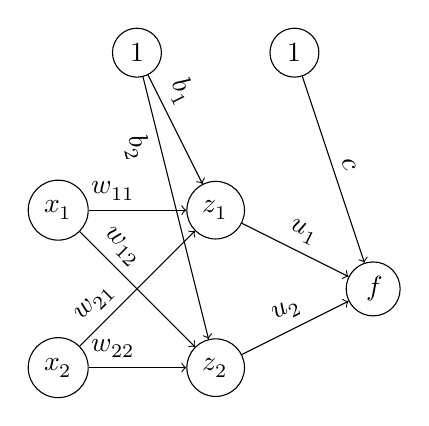
\begin{tikzpicture}
\node[draw,circle] (b1) at (1, 4) {$1$ };
\node[draw,circle] (x1) at (0, 2) {$x_1$ };
\node[draw,circle] (x2) at (0, 0) { $x_2$ };
\node[draw,circle] (b2) at (3, 4) { $1$ };
\node[draw,circle] (z1) at (2, 2) { $z_1$ };
\node[draw,circle] (z2) at (2, 0) { $z_2$ };
\node[draw,circle] (y) at (4, 1) { $f$ };
\draw[->] (b1) -- (z1) node [near start,above,sloped] { $b_1$ };
\draw[->] (b1) -- (z2) node [near start,below,sloped] { $b_2$ };
\draw[->] (x1) -- (z1) node [near start,above,sloped] { $w_{11}$ };
\draw[->] (x1) -- (z2) node [near start,above,sloped] { $w_{12}$ };
\draw[->] (x2) -- (z1) node [near start,above,sloped] { $w_{21}$ };
\draw[->] (x2) -- (z2) node [near start,above,sloped] { $w_{22}$ };
\draw[->] (b2) -- (y) node [midway,above,sloped] { $c$ };
\draw[->] (z1) -- (y) node [midway,above,sloped] { $u_1$ };
\draw[->] (z2) -- (y) node [midway,above,sloped] { $u_2$ };
\end{tikzpicture}
\caption{Structure of the neural network.}
\label{fig:ex1net}
\end{figure}

\begin{Shaded}
\begin{Highlighting}[]
\CommentTok{\# the two input nodes}
\NormalTok{x1 }\OtherTok{=} \FunctionTok{n.var}\NormalTok{(}\StringTok{"x1"}\NormalTok{)}
\NormalTok{x2 }\OtherTok{=} \FunctionTok{n.var}\NormalTok{(}\StringTok{"x2"}\NormalTok{)}

\CommentTok{\# parameters for the first hidden neuron}
\NormalTok{b1 }\OtherTok{=} \FunctionTok{n.var}\NormalTok{(}\StringTok{"b1"}\NormalTok{)}
\NormalTok{w11 }\OtherTok{=} \FunctionTok{n.var}\NormalTok{(}\StringTok{"w11"}\NormalTok{)}
\NormalTok{w21 }\OtherTok{=} \FunctionTok{n.var}\NormalTok{(}\StringTok{"w21"}\NormalTok{)}

\CommentTok{\# compute the output of the first hidden neuron}
\NormalTok{z1in }\OtherTok{=} \FunctionTok{n.sum}\NormalTok{(}
\NormalTok{    b1,}
    \FunctionTok{n.sum}\NormalTok{(}
       \FunctionTok{n.mul}\NormalTok{(x1, w11),}
       \FunctionTok{n.mul}\NormalTok{(x2, w21)))}

\NormalTok{z1out }\OtherTok{=} \FunctionTok{n.tanh}\NormalTok{(z1in)}

\FunctionTok{print.node}\NormalTok{(z1out)}
\end{Highlighting}
\end{Shaded}

Now, complete the remaining part of the network:

\begin{Shaded}
\begin{Highlighting}[]
\CommentTok{\# }\AlertTok{TODO}\CommentTok{ define the parameters of the second hidden neuron}

\NormalTok{z2out }\OtherTok{=}\NormalTok{ (}
  \CommentTok{\# }\AlertTok{TODO}\CommentTok{ compute the output of the second hidden neuron}
\NormalTok{)}

\CommentTok{\# }\AlertTok{TODO}\CommentTok{ define the parameters of the output neuron}

\NormalTok{fin }\OtherTok{=}\NormalTok{ (}
  \CommentTok{\# }\AlertTok{TODO}\CommentTok{ compute the input to the sigmoid (called logits)}
\NormalTok{)}

\NormalTok{fout }\OtherTok{=}\NormalTok{ (}
  \CommentTok{\# }\AlertTok{TODO}\CommentTok{ compute the output of the network: sigmoid(fin)}
\NormalTok{)}

\FunctionTok{print.node}\NormalTok{(fout)}
\end{Highlighting}
\end{Shaded}

And this defines the forward pass.

We can now compute the predictions of the network by evaluating
\texttt{fout}, providing values for the inputs and weights. For example:

\begin{Shaded}
\begin{Highlighting}[]
\FunctionTok{compute}\NormalTok{(z1out, }\FunctionTok{list}\NormalTok{(}
  \CommentTok{\# values for weights and biases}
  \AttributeTok{b1 =} \FloatTok{1.543385}\NormalTok{, }\AttributeTok{w11 =} \FloatTok{3.111573}\NormalTok{, }\AttributeTok{w12 =} \SpecialCharTok{{-}}\FloatTok{2.808800}\NormalTok{,}
  \AttributeTok{b2 =} \FloatTok{1.373085}\NormalTok{, }\AttributeTok{w21 =} \FloatTok{3.130452}\NormalTok{, }\AttributeTok{w22 =} \SpecialCharTok{{-}}\FloatTok{2.813466}\NormalTok{,}
  \AttributeTok{c =} \SpecialCharTok{{-}}\FloatTok{4.241453}\NormalTok{, }\AttributeTok{u1 =} \FloatTok{4.036489}\NormalTok{, }\AttributeTok{u2 =} \FloatTok{4.074885}\NormalTok{,}
  
  \CommentTok{\# values for the input}
  \AttributeTok{x1 =} \DecValTok{1}\NormalTok{, }\AttributeTok{x2 =} \SpecialCharTok{{-}}\DecValTok{1}
\NormalTok{))}
\end{Highlighting}
\end{Shaded}

Which should be about 0.9. We now have to compute the cross-entropy
loss. For numerical stability, we will compute the loss using \(f_{in}\)
instead of \(f_{out}\). Therefore, first, show that:

\begin{equation}
-y\cdot\log(f_{out})-(1-y)\cdot\log(1-f_{out})=
f_{in}-f_{in}\cdot y+\log(1+e^{-f_{in}})
\end{equation}

Solution:

\begin{align}
&-y\cdot\log (f_{out})-(1-y)\cdot\log(1-f_{out}) \\
&\qquad=-y\cdot\log\frac{1}{1+e^{-f_{in}}}-(1-y)\cdot\log\left(1-\frac{1}{1+e^{-f_{in}}}\right) \\
&\qquad=
-y\cdot-\log\left(1+e^{-f_{in}}\right)
-(1-y)\cdot\left(-f_{in}-\log\left(1+e^{-f_{in}}\right)\right) \\
&\qquad=
y\cdot\log\left(1+e^{-f_{in}}\right)
+f_{in}+\log\left(1+e^{-f_{in}}\right)
-y\cdot f_{in}-y\cdot\log\left(1+e^{-f_{in}}\right) \\
&\qquad=f_{in}-f_{in}\cdot y+\log(1+e^{-f_{in}})
\end{align}

\begin{Shaded}
\begin{Highlighting}[]
\CommentTok{\# this variable contains the label for the sample the network is predicting}
\NormalTok{y }\OtherTok{=} \FunctionTok{n.var}\NormalTok{(}\StringTok{"y"}\NormalTok{)}

\NormalTok{loss }\OtherTok{=}\NormalTok{ (}
  \CommentTok{\# }\AlertTok{TODO}\CommentTok{ compute the binary cross entropy loss with the logits (Eq. 3, right)}
\NormalTok{)}

\FunctionTok{print.node}\NormalTok{(loss)}
\end{Highlighting}
\end{Shaded}

This is starting to look complicated! Luckily, this time, we do not have
to get our hands dirty with derivatives; let us find the graphs for the
derivatives of each parameter of the network

\begin{Shaded}
\begin{Highlighting}[]
\NormalTok{param\_names }\OtherTok{=} \FunctionTok{c}\NormalTok{(}\StringTok{"b1"}\NormalTok{, }\StringTok{"w11"}\NormalTok{, }\StringTok{"w12"}\NormalTok{, }\StringTok{"b2"}\NormalTok{, }\StringTok{"w21"}\NormalTok{, }\StringTok{"w22"}\NormalTok{, }\StringTok{"c"}\NormalTok{, }\StringTok{"u1"}\NormalTok{, }\StringTok{"u2"}\NormalTok{)}

\NormalTok{gradient\_graphs }\OtherTok{=} \FunctionTok{lapply}\NormalTok{(param\_names, }\ControlFlowTok{function}\NormalTok{(p) \{}
  \CommentTok{\# each item contains a computational graph that computes}
  \CommentTok{\# the gradient of the loss with respect to a parameter}
  \FunctionTok{simplify}\NormalTok{(}\FunctionTok{differentiate}\NormalTok{(loss, p))}
\NormalTok{\})}

\FunctionTok{names}\NormalTok{(gradient\_graphs) }\OtherTok{=}\NormalTok{ param\_names}

\FunctionTok{print.node}\NormalTok{(gradient\_graphs}\SpecialCharTok{$}\NormalTok{w11)}
\end{Highlighting}
\end{Shaded}

As you can see, there is a great deal of repetition in this expression.
The repetitions could be removed by storing, in each node, its current
value and gradient, so that we would not need to re-compute them every
time. Modern deep learning frameworks indeed do this, and are able to
compute the gradient of the loss with respect to all parameters in a
single pass, but here we accept these inefficiencies for the sake of
simplicity.

We are now ready to train this network:

\begin{Shaded}
\begin{Highlighting}[]
\CommentTok{\# dataset}
\NormalTok{data.x1 }\OtherTok{=} \FunctionTok{c}\NormalTok{(}\DecValTok{0}\NormalTok{, }\DecValTok{1}\NormalTok{, }\DecValTok{0}\NormalTok{, }\SpecialCharTok{{-}}\DecValTok{1}\NormalTok{, }\DecValTok{0}\NormalTok{)}
\NormalTok{data.x2 }\OtherTok{=} \FunctionTok{c}\NormalTok{(}\DecValTok{0}\NormalTok{, }\DecValTok{0}\NormalTok{, }\SpecialCharTok{{-}}\DecValTok{1}\NormalTok{, }\DecValTok{0}\NormalTok{, }\DecValTok{1}\NormalTok{)}
\NormalTok{data.y }\OtherTok{=} \FunctionTok{c}\NormalTok{(}\DecValTok{1}\NormalTok{, }\DecValTok{0}\NormalTok{, }\DecValTok{0}\NormalTok{, }\DecValTok{0}\NormalTok{, }\DecValTok{0}\NormalTok{)}

\CommentTok{\# Glorot initializtion for the parameters}
\NormalTok{b }\OtherTok{=} \FunctionTok{sqrt}\NormalTok{(}\DecValTok{6} \SpecialCharTok{/} \DecValTok{4}\NormalTok{)}
\NormalTok{values }\OtherTok{=} \FunctionTok{as.list}\NormalTok{(}\FunctionTok{sapply}\NormalTok{(param\_names, }\ControlFlowTok{function}\NormalTok{(p) \{}
  \ControlFlowTok{if}\NormalTok{(p }\SpecialCharTok{\%in\%} \FunctionTok{c}\NormalTok{(}\StringTok{"b1"}\NormalTok{, }\StringTok{"b2"}\NormalTok{, }\StringTok{"c"}\NormalTok{)) \{}
    \FloatTok{0.0}
\NormalTok{  \}}
  \ControlFlowTok{else}\NormalTok{ \{}
    \FunctionTok{runif}\NormalTok{(}\DecValTok{1}\NormalTok{, }\SpecialCharTok{{-}}\NormalTok{b, b)}
\NormalTok{  \}}
\NormalTok{\}))}

\CommentTok{\# training loop}
\NormalTok{losses }\OtherTok{=} \FunctionTok{list}\NormalTok{()}
\ControlFlowTok{for}\NormalTok{(e }\ControlFlowTok{in} \DecValTok{0}\SpecialCharTok{:}\DecValTok{250}\NormalTok{) \{}
\NormalTok{  epoch\_loss }\OtherTok{=} \FloatTok{0.0}
  
  \ControlFlowTok{for}\NormalTok{(j }\ControlFlowTok{in} \DecValTok{1}\SpecialCharTok{:}\DecValTok{5}\NormalTok{) \{}
    \CommentTok{\# set the correct values for the inputs and label}
\NormalTok{    values}\SpecialCharTok{$}\NormalTok{x1 }\OtherTok{=}\NormalTok{ data.x1[j]}
\NormalTok{    values}\SpecialCharTok{$}\NormalTok{x2 }\OtherTok{=}\NormalTok{ data.x2[j]}
\NormalTok{    values}\SpecialCharTok{$}\NormalTok{y }\OtherTok{=}\NormalTok{ data.y[j]}

\NormalTok{    losses[[e }\SpecialCharTok{*} \DecValTok{5} \SpecialCharTok{+}\NormalTok{ j]] }\OtherTok{=}\NormalTok{ (}
      \CommentTok{\# }\AlertTok{TODO}\CommentTok{ compute the loss for sample j}
\NormalTok{    )}
    
\NormalTok{    gradients }\OtherTok{=} \FunctionTok{sapply}\NormalTok{(param\_names, }\ControlFlowTok{function}\NormalTok{(p) \{}
      \CommentTok{\# }\AlertTok{TODO}\CommentTok{ compute the gradient for parameter p}
\NormalTok{    \})}
    
\NormalTok{    values }\OtherTok{=} \FunctionTok{as.list}\NormalTok{(}\FunctionTok{sapply}\NormalTok{(param\_names, }\ControlFlowTok{function}\NormalTok{(p) \{}
      \CommentTok{\# }\AlertTok{TODO}\CommentTok{ update parameter p with one step of gradient descent}
\NormalTok{    \}))}
\NormalTok{  \}}
\NormalTok{\}}

\FunctionTok{stopifnot}\NormalTok{(}\FunctionTok{mean}\NormalTok{(}\FunctionTok{unlist}\NormalTok{(}\FunctionTok{tail}\NormalTok{(losses))) }\SpecialCharTok{\textless{}} \FloatTok{0.05}\NormalTok{) }\CommentTok{\# convergence check (sometimes fails)}
\FunctionTok{plot}\NormalTok{(}\DecValTok{1}\SpecialCharTok{:}\FunctionTok{length}\NormalTok{(losses), losses)}
\end{Highlighting}
\end{Shaded}

You can clearly see how the loss of each individual training sample
evolves over time. This also explains the ``saddle'' you might have
noticed in the loss curve from the previous lab.

And these are the predictions for the five points:

\begin{Shaded}
\begin{Highlighting}[]
\ControlFlowTok{for}\NormalTok{(j }\ControlFlowTok{in} \DecValTok{1}\SpecialCharTok{:}\DecValTok{5}\NormalTok{) \{}
\NormalTok{  values}\SpecialCharTok{$}\NormalTok{x1 }\OtherTok{=}\NormalTok{ data.x1[j]}
\NormalTok{  values}\SpecialCharTok{$}\NormalTok{x2 }\OtherTok{=}\NormalTok{ data.x2[j]}
\NormalTok{  values}\SpecialCharTok{$}\NormalTok{y }\OtherTok{=}\NormalTok{ data.y[j]}

\NormalTok{  pred }\OtherTok{=} \FunctionTok{compute}\NormalTok{(fout, values)}
  \FunctionTok{cat}\NormalTok{(}\StringTok{"Sample"}\NormalTok{, j, }\StringTok{"{-}"}\NormalTok{, }\StringTok{"label:"}\NormalTok{, data.y[j], }\StringTok{"{-} predicted: "}\NormalTok{, pred, }\StringTok{"}\SpecialCharTok{\textbackslash{}n}\StringTok{"}\NormalTok{)}
\NormalTok{\}}
\end{Highlighting}
\end{Shaded}

\hypertarget{conclusion}{%
\subsubsection{Conclusion}\label{conclusion}}

What we did in this exercise is (a simplification of) how deep learning
frameworks evaluate the code you write. You only need to define how to
compute the output of the network, and the framework figures out the
necessary gradients on its own. They provide a much better user
interface, allowing you to use \texttt{+}, \texttt{-}, \texttt{/},
\texttt{*} etc. as you normally would instead of the clumsy node
constructors we defined here, but there is always a computational graph
hidden behind the curtains.

\hypertarget{exercise-2}{%
\subsection{Exercise 2}\label{exercise-2}}

This exercise should improve your understanding of weight decay (or L2
regularization).

\begin{enumerate}
\def\labelenumi{\arabic{enumi}.}
\item
  Consider a quadratic error function
  \(E(\textbf{w})=E_0+\textbf{b}^T\textbf{w}+1/2\cdot\textbf{w}^T\textbf{H}\textbf{w}\)
  and its regularized counterpart
  \(E'(\textbf{w})=E(\textbf{w})+\tau/2 \cdot\textbf{w}^T\textbf{w}\),
  and let \(\textbf{w}^*\) and \(\tilde{\textbf{w}}\) be the minimizers
  of \(E\) and \(E'\) respectively. We want to find a node to express
  \(\tilde{\textbf{w}}\) as a function of \(\textbf{w}^*\), i.e.~find
  the displacement introduced by weight decay.

  \begin{itemize}
  \tightlist
  \item
    Find the gradients of \(E\) and \(E'\). Note that, at the global
    minimum, we have
    \(\nabla E(\textbf{w}^*)=\nabla E'(\hat{\textbf{w}})=0\).
  \item
    In the equality above, express \(\textbf{w}^*\) and
    \(\tilde{\textbf{w}}\) as a linear combination of the eigenvectors
    of \(\textbf{H}\).
  \item
    Through algebraic manipulation, obtain \(\tilde{\textbf{w}}_i\) as a
    function of \(\textbf{w}^*_i\).
  \item
    Interpret this result geometrically.
  \item
    Note: \(\textbf{H}\) is square, symmetric, and positive definite,
    which means that its eigenvectors are pairwise orthogonal and its
    eigenvalues are positive (spectral theorem).
  \end{itemize}
\item
  Consider a linear network of the form \(y=\textbf{w}^T\textbf{x}\) and
  the mean squared error as a loss function. Assume that every
  observation is corrupted with Gaussian noise
  \(\epsilon\sim\mathcal{N}(\textbf{0}, \sigma^2\textbf{I})\). Compute
  the expectation of the gradient under \(\epsilon\) and, show that
  adding gaussian noise to the inputs has the same effect of weight
  decay.
\end{enumerate}

\end{document}
